\documentclass[12pt,letterpaper]{exam}
\usepackage[utf8]{inputenc}
\usepackage[T1]{fontenc}
\usepackage[width=8.50in, height=11.00in, left=0.50in, right=0.50in, top=0.50in, bottom=0.50in]{geometry}

\usepackage{libertine}
\usepackage{multicol}
\usepackage[shortlabels]{enumitem}

\usepackage{booktabs}
\usepackage[table]{xcolor}

\usepackage{amssymb}
\usepackage{amsthm}
\usepackage{mathtools}
\usepackage{bbm}

\usepackage{hyperref}
\usepackage{graphicx}
%\usepackage{wrapfig}
%\usepackage{capt-of}
\usepackage{tikz}
%\usepackage{pgfplots}
\usetikzlibrary{shapes,arrows,positioning,patterns}
%\usepackage{pythonhighlight}

%\newcommand\chapter{5}
%\renewcommand{\thequestion}{\textbf{\chapter.\arabic{question}}}
\renewcommand{\questionlabel}{\textbf{\thequestion}.}

%%%%%%%%%%%%%%%%%%%%%%%%%%%%%%%%%%%%%%%%%%%%%%%%%%%%%%%%%%%%%%%%%%
\newcommand{\class}{STAT 601} % This is the name of the course 
\newcommand{\assignmentname}{Midterm 2 Redux} % 
\newcommand{\authorname}{Hosley, Brandon} % 
\newcommand{\workdate}{\today} % 
\printanswers % this includes the solutions sections
%%%%%%%%%%%%%%%%%%%%%%%%%%%%%%%%%%%%%%%%%%%%%%%%%%%%%%%%%%%%%%%%%%



\begin{document}
\pagestyle{plain}
\thispagestyle{empty}
\noindent
 
%%%%%%%%%%%%%%%%%%%%%%%%%%%%%%%%%%%%%%%%%%%%%%%%%%%%%%%%%%%%%%%%%%%%%%%%%%%%%%%%%%%
\noindent
\begin{tabular*}{\textwidth}{l @{\extracolsep{\fill}} r @{\extracolsep{10pt}} l}
	\textbf{\class} & \textbf{\authorname}  &\\ %Your name here instead, obviously 
	\textbf{\assignmentname } & \textbf{\workdate} & \\
\end{tabular*}\\ 
\rule{\textwidth}{2pt}
%%%%%%%%%%%%%%%%%%%%%%%%%%%%%%%% HEADER %%%%%%%%%%%%%%%%%%%%%%%%%%%%%%%%%%%%%%%%%%%

\begin{questions}

	\setcounter{question}{0}
	\question 
	\textbf{(30 points)}  \(f_{Y|X}(y|x) = \frac{2y}{x^2}\mathbbm{1}_{(0,x)}(y) \) and \(f_{X}(x) = 5x^4\mathbbm{1}_{(0,1)}(x) \)
	
	\begin{parts}
	\setcounter{partno}{3}
		\part Given \(X\) is less than \(\frac{1}{2}\), what is the probability that \(Y\) is less than \(\frac{1}{4}\)?
	\end{parts}

	\begin{solution}
		Using the property,
		\[ f_{Y|X} = \frac{f_{YX}(y,x)}{f_X(x)} \Rightarrow f_{Y|X}\left(\left.y<\frac{1}{4}\right|x<\frac{1}{2}\right) = \frac{f_{YX}(y<\frac{1}{4},x<\frac{1}{2})}{f_X(x<\frac{1}{2})}. \]
		First,
		\[ P\left(x<\frac{1}{2}\right) = \int_{0}^{\frac{1}{2}} 5x^4 \,dx =  x^5 \Big|_{0}^\frac{1}{2} = \left(\frac{1}{2}\right)^5. \]
		Next, \(f_{YX}\) noting that there will be two sets of bounds,
		\begin{align*}
			\int_{0}^{\frac{1}{4}} \int_{0}^{x} 10yx^2\,dy\,dx	&+ \int_{\frac{1}{4}}^{\frac{1}{2}} \int_{0}^{\frac{1}{4}} 10yx^2\,dy\,dx \\
			\left[5\right]\times\quad  \int_{0}^{\frac{1}{4}} x^2 \Big[y^2\Big]_0^x \,dx	&+ \int_{\frac{1}{4}}^{\frac{1}{2}} x^2 \Big[y^2\Big]_0^\frac{1}{4} \,dx \\
			\left[5\right]\times\qquad  \int_{0}^{\frac{1}{4}} x^4 \,dx	&+ \int_{\frac{1}{4}}^{\frac{1}{2}} x^2 \left(\frac{1}{4}\right)^2 \,dx \\
			\left[5\right]\times\qquad \left.\left(\frac{1}{5}\right) x^5\right|_{0}^{\frac{1}{4}} 	
				&+	\left(\frac{1}{4}\right)^2 \left.\left(\frac{1}{3}\right)x^3\right|_{\frac{1}{4}}^{\frac{1}{2}}  \\
			\left[5\right]\times\qquad\left(\frac{1}{5}\right) \left(\frac{1}{4}\right)^5
			&+	\left(\frac{1}{4}\right)^2 \left(\frac{1}{3}\right) \left[ \left(\frac{1}{2}\right)^3 -\left(\frac{1}{4}\right)^3 \right]  \\
			\left[5\right]\times\qquad \frac{1}{5(4)^5} &+ \frac{1}{3(2)^4} \left( \frac{1}{8} - \frac{1}{64} \right) \\
			\left[5\right]\times\quad \left( \frac{1}{5(2)^{10}} \right. &+ \left. \frac{7}{3(2)^6} \right) \\
			5 \left( \frac{3+35}{15(2)^{10}} \right)& \\
			\frac{38}{3(2)^{10}} & \\
		\intertext{we divide by the \(f_X(x)\) from above,}
			\frac{38}{3(2)^{5}} = \frac{19}{3(2)^{4}} =& \frac{19}{48}. \\
		\end{align*}
		
	\end{solution} \clearpage
	%%%%%%%%%%%%%%%%%%%%%%%%%%%%%%%%%%%%%%%%%%%%%%%%%%%%%%%%%%%%%

	\question 
	\textbf{(30 points)}  Let both \(X_1, X_2\) be independent \(POI(\lambda)\) random variables. Define \(Y = X_1 + X_2\).
	
	\begin{parts}
		\part Derive and identify the distribution of \(Y\). Give the form of its pdf, \(f_Y(y)\)
	\end{parts}
	
	\begin{solution}
		Using the property that, when \(Y=X_1+X_2\)
		\begin{align*}
			\text{MGF}_Y(t) 
			&= \text{MGF}_{X_1}(t) \text{MGF}_{X_2}(t) \\
			&= e^{\lambda(e^t-1)} \, e^{\lambda(e^t-1)} \\
			&= e^{2\lambda(e^t-1)} \\ 
			\therefore&\sim\text{Poi}(2\lambda)
		\end{align*}
		and we also determine that \(f_Y(y) = \frac{2\lambda^ye^{-2\lambda}}{y!}\).
		
	\end{solution}
	%%%%%%%%%%%%%%%%%%%%%%%%%%%%%%%%%%%%%%%%%%%%%%%%%%%%%%%%%%%%%
	
	\question 
	\textbf{(30 points)} : Let \(X\) be the number obtained from a single roll of a fair 8 sided die.
	Given the value of \(X\), roll a second fair die with \(x\) sides, numbered \(1,2,\ldots,x\).
	Let \(Y\) denote the number obtained on the roll of the second die.
	The joint pmf is:
	\begin{flalign*} \qquad
		f_{XY}(x,y) = \begin{cases}
			\frac{1}{8x} & x= 1,2,\ldots,8;\ y = 1,2,\ldots,x \\
			0 & \text{otherwise.}
		\end{cases} &&
	\end{flalign*}
	
	\begin{parts}
		\part Evaluate \(P(Y>X-3)\).
	\end{parts}
	
	\begin{solution}
		Solving by brute force, as below, without trying to be fancy, we see $P(Y>X-3) = \frac{21}{36}$.
		
		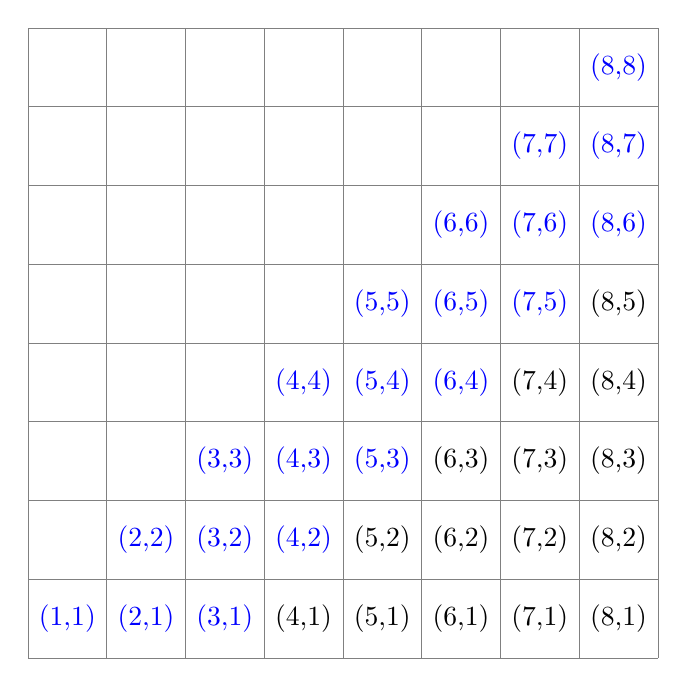
\begin{tikzpicture}
			% Draw the grid
			\draw[step=1cm, gray, very thin] (0,0) grid (8,8);
			
			% Loop through x and y coordinates
			\foreach \x in {1,...,8} {
				\foreach \y in {1,...,8} {
					% Check if y <= x
					\ifnum\y>\x\relax
					% Do nothing
					\else
					% Place the coordinate text
						% Check if y > x - 3
						\pgfmathparse{\y > \x - 3 ? int(1) : int(0)}
						\ifnum\pgfmathresult=1
						\node at (\x-0.5, \y-0.5) {\textcolor{blue}{(\x,\y)}};
						\else
						\node at (\x-0.5, \y-0.5) {(\x,\y)};
						\fi
					\fi
				}
			}
		\end{tikzpicture}
	\end{solution}
	%%%%%%%%%%%%%%%%%%%%%%%%%%%%%%%%%%%%%%%%%%%%%%%%%%%%%%%%%%%%%
		

\end{questions}
\end{document}
